%!TEX root =  Report.tex
\chapter{Tutorial}
\section{Introduction}

Let me get back to you on taht one
%TODO: get back to this one

\section{The Very Basics}

The {\tt drul} command can take DruL code either from the standard input or as a file specified on the command line ({\tt drul mysource.drul}).  Examples in this section should work equally well if passed in either way.

\subsection{Say hello!}

Because it is traditional, albeit almost completely irrelevant to this language, here is our first
DruL program:

\begin{lstlisting}
print("hello, world!");
\end{lstlisting}

This will print the string ``hello, world!'' to the standard output, on a line by itself.  Note that unlike many languages, DruL does not require you to place a newline character at the end of a string to have it print on a single line (conversely, it gives you no method to print \emph{without} a newline at the end).

\subsection{Fundamentals}

Variables in DruL must have names that begin with a letter or underscore, and contain only letters, numbers, and underscores thereafter.  Variables are dynamically typed and scoped, so to create one, you need only assign a value to it:

\begin{lstlisting}
a = 350;
b = 300;
print(a + b);
\end{lstlisting}

This should print out the number ``650'', again on a line by itself.

Now, with some variables defined, we can proceed quickly through the rest of the features that
you might guess are present from the above:


\begin{lstlisting}
a = 350;
b = 300;

c = b - a;

d = a % b;

e = 60 / d;

if (e > 1) {
	print("this is what you might expect to have happen");
} else {
	print("but this is what actually prints");
}

\end{lstlisting}

Why does the second line print, and not the first?  DruL's types do not include floating-point numbers, so all arithmetic is done using integers, and non-integral results are truncated (as is done in C and other related languages) to their integer parts.

\subsection{One more variable type: patterns}

We will now introduce the first data type that distinguishes DruL from most other languages: the pattern.  A pattern is a sequence of true/false values, telling the drummer (or MIDI sequencer) whether or not to play on a particular beat.  They are created using the {\tt pattern} function:

\begin{lstlisting}
p1 = pattern("");	 // empty pattern (length 0)
p2 = pattern("0");       // pattern with only one 'rest' in it.
p3 = pattern("1");       // pattern with only one 'note' in it.
p4 = pattern("100100100");
\end{lstlisting}

Each time a ``1'' appears in the string you pass to {\tt pattern}, the resulting pattern carries the instruction to play on that beat; when a ``0'' appears, the pattern contains a rest.
You may notice that we also have explanatory comments in this code: comments in DruL begin with ``//'' and continue to the end of the current line (there are no multi-line comments).

To see the contents of a pattern you have created, you can always just print it out:

\begin{lstlisting}
p = pattern("100100100");
print(p);
\end{lstlisting}


\section{Combining Patterns}

Once you have a pattern or two, DruL gives you several ways to build new ones.  Using the {\tt concat} function, you can combine them end-to-end:
\begin{lstlisting}
catenated = concat(
	p1,
	pattern("11110000"),
	pattern("00011")
);
\end{lstlisting}
Notice that we have broken up the arguments to {\tt concat} onto multiple lines for ease of reading--since DruL is a free-form language, any amount of whitespace can appear any place that any whitespace is allowed.

Pattern objects also have a {\tt repeat} method, which produces a new pattern containing all the beats and rests of the original, repeated however many times the method is given as its argument.  (In fact, you can give it an argument of 0 to return an empty pattern, though there are less obscure ways to do that.)

\begin{lstlisting}
p_custom = concat(
	p2,
	p3.repeat(2),
	p4.repeat(3),
	p3.repeat(2),
	p4.repeat(4)
);
\end{lstlisting}
\section{Manipulating Patterns}

Patterns also have methods that allow you to produce new patterns that are not simply combinations of old ones laid end to end.

Using the {\tt reverse} method, you can turn a pattern back to front; using the {\tt slice} method, you can extract just the portion of it you want:

\begin{lstlisting}
bassackwards = catenated.reverse();

p_new = bassackwards.slice(4,10);
\end{lstlisting}

The arguments to {\tt slice} tell DruL which is the first beat of the pattern that you're interested in, and how many beats (including that one) you would like.  So to the call above will produce a pattern 10 beats long, that starts with the 4th beat of {\tt bassackwards}.  If you ask for more beats than the pattern has, then {\tt slice} will return a pattern that starts on the beat you specify and continues until the end of the original pattern.

Since all of these methods return patterns, and are methods of patterns, you can also stack your method calls into one statement:

\begin{lstlisting}
p_new = catenated.reverse().slice(4,10);
\end{lstlisting}

But the most powerful mechanism for creating new and different patterns is the {\tt map} function.  This is how to take a pattern and create its complement: a pattern that has a rest everywhere that the original has a note, and vise-versa:

\begin{lstlisting}
reversed = map (p_new) {
	if ($1.rest()) { return pattern("1"); }
	else 	       { return pattern("0"); }
};
\end{lstlisting}

The {\tt map} function moves from beat to beat of the pattern it is passed, setting the variable {\tt \$1} to the point to the current beat of the first (and in this case, the only) pattern in its argument list.  After each step, it stores the value that is returned, and in the end, it concatenates all these patterns together to form the new pattern that is created by this map.

You might be wondering, at this point, if it is legal to return a pattern that is longer or shorter than one beat.  The answer, happily, is ``yes!''  To produce, for example, a pattern that has an extra rest inserted after every note, we could do this:

\begin{lstlisting}
new_pattern = map(old_pattern) {
	if ( $1.note() ) { return pattern("10"); }
	return $1;
};
\end{lstlisting}
You may notice that we didn't bother to create a pattern for the second case: if we simply want to return a single-beat pattern with the same value (beat or rest) as the current beat of one of our input patterns, we can simply return that beat, and DruL will interpret it correctly.

Finally, we can pass more than one pattern to a mapper, and use variables {\tt \$2}, {\tt \$3} and so forth.  This mapper takes two patterns as its arguments, and produces a new pattern that contains the portions of the first pattern that occur in parallel with notes (not rests) in the second pattern:
\begin{lstlisting}
old_pattern = pattern("10101100");
filtered_pattern = map(old_pattern, pattern("1110011110000") ) {
	if ( $2.note() ) { return $1; }
};
print(old_pattern);
\end{lstlisting}
In this case, the printed value will be ``101100'' (if no return statement is found, {\tt map} assumes that you meant to return an empty pattern).
The same result could be achieved using a series of calls to {\tt slice} and {\tt concat}, but this is a much more flexible method.

If one of the patterns passed to {\tt map} is longer than the others, {\tt map} will continue until it reaches the end of the longest pattern--the beats of the patterns that have already ended are considered to be neither notes nor rests (and will return false if either of those methods is called).

We've mentioned beats as if they were objects once or twice, and in fact they are--you can't create them directly, but {\tt map} does it for you.  You've seen two of the methods you can call on beats ({\tt note} and {\tt rest}, but there are two more that make {\tt map} even more powerful:  {\tt prev} and {\tt next}.
Calling {\tt prev} with an integer argument returns the beat in the same pattern from that many beats ago in the pattern (and you can probably guess how {\tt next} works).  These beats may be from before the beginning or after the end of the pattern, in which case they behave just as described in the previous paragraph: both the {\tt note} and {\tt rest} methods will return {\tt false}.

\begin{lstlisting}
new_pattern = map (old_pattern) {
	if ( $1.note() && $1.prev(1).note() ) { return $1; }
	else { return pattern(""); }
};
\end{lstlisting}

\section{Named mappers}

In all of the examples so far, we have simply supplied the {\tt map} function with a block of statements to run for this particular set of patterns.  This block is what we refer to as an ``anonymous mapper.''  In reality, of course, it is likely you would want perform the same type of transformation on more than one pattern (or set of patterns).  To do this without annoying repetition of code, you can define a named mapper, then use the name instead of the code block.  The named mapper can also have named parameters, which may be easier to keep track of than the shell-like variables used in anonymous mappers.  This allows us to re-write the previous example in a somewhat more readable way:
\begin{lstlisting}
mapper filter_map ( input_pattern, filter_pattern ) {
	if ( filter_pattern.note() ) { return input_pattern; }
};

filtered_pattern =
	map (old_pattern, pattern("1110011110000") ) filter_map;
\end{lstlisting}



\section{Assembling clips}

Now that we have a bunch of patterns, the next thing to do with them is assemble them into pieces of music, where each instrument has a (presumably) different pattern to play.  Before we do that, however, we have to define what instruments we are using.  This is done using the {\tt instruments} function (which isn't actually a function at all, but we're going to ignore that for now--see section \ref{instrSection} in the Language Reference Manual if you want the grizzly details).
\begin{lstlisting}
instruments("hihat","bassdrum","crash","snare");
\end{lstlisting}
If you want to use the default instruments, you can simply call {\tt instruments} with no arguments, but you have to call it once (and exactly once) before you get to the next step: using the {\tt clip} function to bring all of your patterns into one place.
\begin{lstlisting}
my_first_clip = clip(
	"hihat" <- pattern("00100010"),
	"bassdrum" <- pattern("10001000"),
	"crash" <- pattern("10000000"),
	"snare" <- pattern("01110111")
);
\end{lstlisting}
Of course, this is a little verbose--if you're specifying the patterns in the order they appear in the instrument definition list, you can just pass the patterns you want as arguments, instead of using the fancy syntax above:
\begin{lstlisting}
my_first_clip = clip(
	pattern("00100010"),
	pattern("10001000"),
	pattern("10000000"),
	pattern("01110111")
);
\end{lstlisting}

\section{The Big Payoff}
Now that we know how to assemble patterns into a song, all that's left is to see what our song looks like
when we bring it back to the outside world.  There are three easy ways to do this (other, of course, than a simple {\tt print} call).  First, you can call the {\tt outputText} method to print your song to a text file:
\begin{lstlisting}
instruments();  // default instruments: hihat, snare, kick-drum and cowbell

song = clip(
	pattern("00100010"),
	pattern("01110111"),
	pattern("10001000"),
	pattern("10000000")
);
song.outputText("my_song.txt");
\end{lstlisting}

If you have the {\tt midge} program\footnote{\url{http://www.undef.org.uk/code/midge/}} installed, you can also convert it directly into a MIDI file you can play using many music players:
\begin{lstlisting}
tempo = 120;
song.outputMidi("my_song.mid", 120);
\end{lstlisting}
And finally, you can output to the format used by the typesetting package Lilypond\footnote{\url{http://www.lilypond.org/}}
to produce beautifully typeset  sheet music:
\begin{lstlisting}
song.outputLilypond("my_song.ly", "Title of the Song");
\end{lstlisting}
Assuming you have Lilypond installed, this allows you to produce PDF sheet music that looks roughly like this:

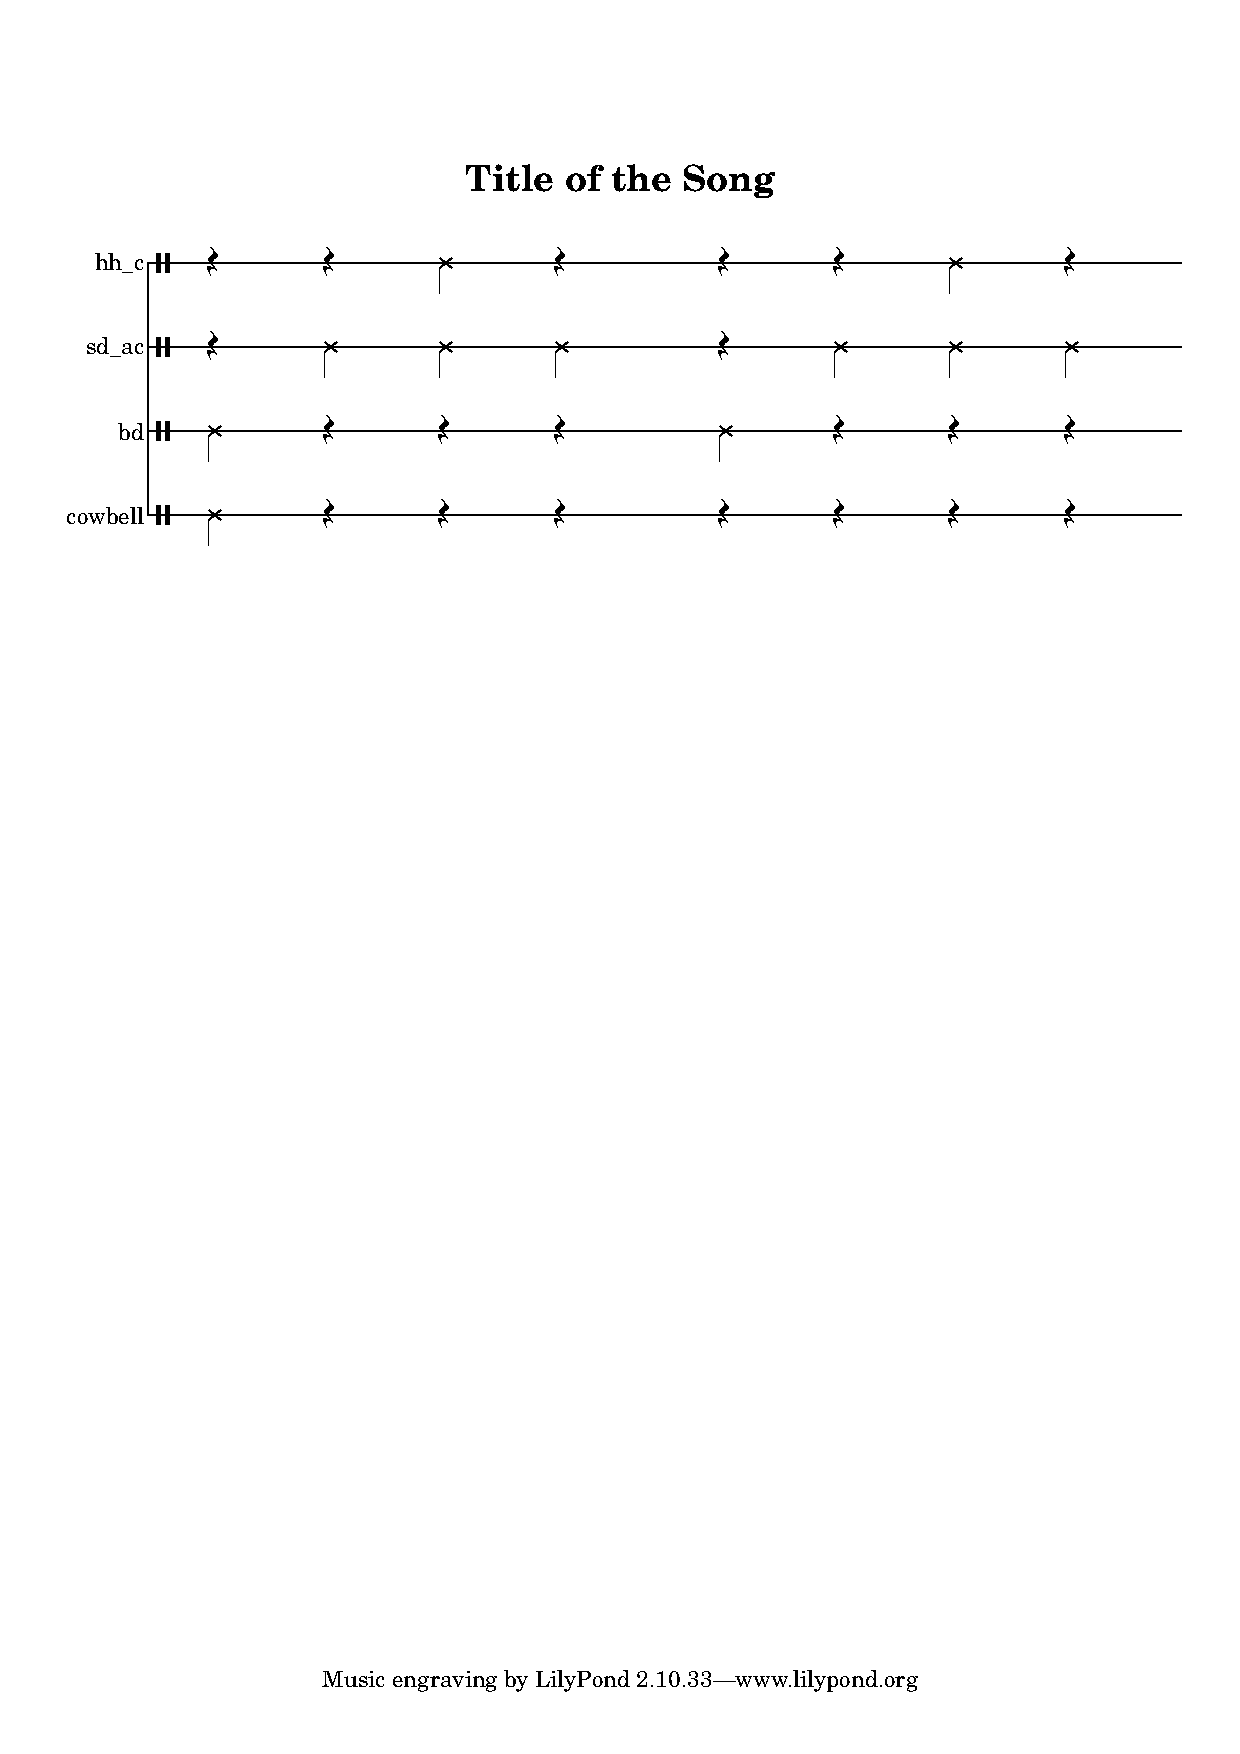
\includegraphics[scale=0.8,trim=1in 7in 0.5in 0.5in]{MYSONG.pdf}

Congratulations!  You're done with the tutorial--have fun with DruL!
